\documentclass[smallextended]{svjour3}

\usepackage{amsfonts}
\usepackage{amsmath}
\usepackage{algorithm,algcompatible}
\usepackage{bbm}
\usepackage{bm}
\usepackage{soul}
\DeclareMathOperator*{\argmax}{arg\,max}
\usepackage{tikz}
\usetikzlibrary{shapes.geometric, arrows}
\usepackage{graphicx}
\usepackage{natbib}
\usepackage{booktabs}
\usepackage{hyperref}

\algnewcommand\INPUT{\item[\textbf{Input:}]}%
\algnewcommand\OUTPUT{\item[\textbf{Output:}]}%
\algnewcommand\textproc{\textsc}
\newcommand{\trnp}{^\text{T}}
\newcommand{\bg}[1]{\textcolor{red}{#1}}



% \raggedbottom

\begin{document}

\title{Estimating Heterogeneous Treatment Effect on Multivariate Responses using Random Forests}
\titlerunning{MULTIPLE OUTCOME TREATMENT EFFECT FOREST}

\author{Boyi Guo \and
        Hannah D. Holscher \and
        Loretta S. Auvil \and
        Michael E. Welge \and
        Colleen B. Bushell \and
        Janet A. Novotny \and 
        David J. Baer \and
        Nicholas A. Burd \and
        Naiman A. Khan \and
        Ruoqing Zhu*
        }
%\authorrunning{Guo et}
%\author[1]{Boyi Guo}
%\author[2,4]{Ruoqing Zhu*}
%\author[3,4]{Hannah D. Holscher}
%\author[4]{Loretta S. Auvil}
%\author[4]{Michael E. Welge}
%\author[4]{Colleen B. Bushell}
%\author[5]{David J. Baer}
%\author[5]{Janet A. Novotny}

%\address[1]{\orgdiv{Department of Biostatistics}, \orgname{School of Public Health}, \orgname{University of Alabama at Birmingham}, \orgaddress{\city{Birmingham}, \state{Alabama}, \country{USA}}}

%\address[2]{\orgdiv{Department of Statistics}, \orgname{University of Illinois at Urbana-Champaign}, \orgaddress{\city{Champaign}, \state{IL}, \country{USA}}}

%\address[3]{\orgdiv{Department of Food Science and Human Nutrition}, \orgname{University of Illinois at Urbana-Champaign}, \orgaddress{\city{Champaign}, \state{IL}, \country{USA}}}

%\address[4]{\orgdiv{National Center for Supercomputing Applications}, \orgname{University of Illinois at Urbana-Champaign}, \orgaddress{\city{Champaign}, \state{IL}, \country{USA}}}

%\address[5]{\orgdiv{USDA}, \orgdiv{Agricultural Research Service}, \orgname{Beltsville Human Nutrition Research Center}, \orgaddress{\city{Beltsville}, \state{MD}, \country{USA}}}

%\corres{*Ruoqing Zhu, Department of Statistics, University of Illinois at Urbana-Champaign, Champaign, IL, USA. \email{rqzhu@illinois.edu}}

\institute{B. Guo \at
           Department of Biostatistics,\\
            University of Alabama at Birmingham,\\
             Birmingham, AL 35244, USA
           \and
           H. Holscher \at
           Department of Food Science and Human Nutrition,\\
           University of Illinois at Urbana-Champaign,\\ 
           Champaign, IL 61801, USA
        \and
        L. S. Auvil \at
        National Center for Supercomputing Applications,\\
        University of Illinois at Urbana-Champaign,\\
        Champaign, IL 61801, USA    
        \and
        M. E. Welge \at
        National Center for Supercomputing Applications,\\
        University of Illinois at Urbana-Champaign,\\
        Champaign, IL 61801, USA        
        \and
        C. B. Bushell \at
        National Center for Supercomputing Applications,\\
        University of Illinois at Urbana-Champaign,\\
        Champaign, IL 61801, USA
        \and 
        J. Novotny \at
        USDA, ARS,\\
        Beltsville Human Nutrition Research Center,\\
        Beltsville, MD 20705, USA
        \and 
        D. Baer \at
        USDA, ARS,\\
        Beltsville Human Nutrition Research Center,\\
        Beltsville, MD 20705, USA
        \and
        N. Burd \at
        Department of Kinesiology and Community Health\\
        University of Illinois at Urbana-Champaign,\\ 
        Champaign, IL 61801, USA
        \and
        N. Khan \at
        Department of Kinesiology and Community Health,\\
        University of Illinois at Urbana-Champaign,\\ 
        Champaign, IL 61801, USA
            \and
           R. Zhu \at
             Department of Statistics,\\
             University of Illinois at Urbana-Champaign,\\ 
             Champaign, IL 61801, USA\\
             \email{rqzhu@illinois.edu}  
}

% \date{Received: date / Accepted: date}

\maketitle

\begin{abstract}
    Estimating the individualized treatment effect has become one of the most popular topics in statistics and machine learning communities in recent years. Most existing methods focus on modeling the heterogeneous treatment effects for univariate outcomes. However, many biomedical studies are interested in studying multiple highly correlated endpoints at the same time. We propose a random forest model that simultaneously estimates individualized treatment effects of multivariate outcomes. We consider a popular study design where covariates and outcomes are measured both before and after the intervention. The proposed model uses oblique splitting rules to partition population space to the neighborhood that experiences distinct treatment effects. An extensive simulation study suggests that the proposed method outperforms existing methods in various nonlinear settings. We further apply the proposed method to two nutrition studies investigating the effects of food consumption on gastrointestinal microbiota composition and clinical biomarkers. The method has been implemented in a freely available R package MOTE.RF at \url{https://github.com/boyiguo1/MOTE.RF}.
\end{abstract}

\keywords{individualized treatment effect \and microbiota \and multivariate \and random forests \and personalized nutrition}

\section{Introduction}\label{Intro}
Precision medicine is a rapidly growing field in statistics and clinical practice. It takes individual heterogeneity, environment, and lifestyles into consideration when making decisions to improve human health. Recent advances in large-scale biomedical databases and computational devices dramatically improve the prospect of optimizing an individual's treatment \citep{Collins2015}. The launch of the Precision Medicine Initiative sparks much more research in discovering individualized treatment. 

As data aggregates from various projects, such as the 100,000 Genome Project \citep{Peplowi1757}, the Personal Genomes Project \citep{ball2014harvard} and many others, the demand for analytic tools has never been higher. Many statistical and machine learning models have been proposed to facilitate data analysis with am emphasis on individualized treatment. Some regression-based methods \citep{Brinkley2010,qian2011performance} model responses as a function of patient characteristics and treatment, and select the treatment that maximizes predicted responses. Scoring systems built with parametric or semi-parametric regression\citep{Cai2011, Zhao2013} are used to identify populations that experience different treatment effects. Policy-search or direct-maximization methods \citep{Zhang2012,zhang2012robust, Zhao2012, Zhang2013} offer an alternative to the regression-based approaches, attempting to find the best rule by directly optimizing an estimator of the overall population mean response. We refer to \cite{kosorok2015adaptive} for a general overview of this field. 

Analyzing biomedical data faces many challenges. When domain knowledge is lacking, distinct model specifications can lead to hugely different estimations. Moreover, violation of parametric assumptions makes inference doubtful. Nevertheless, tree-based methods hold a promising role in addressing these challenges. While they require less model specification, the nonparametric property provides flexibility to explore underlying model structures. Hence, they have been extensively used in applications, such as survival analysis \citep{gordon1985tree, leblanc1992relative, hothorn2005survival, ishwaran2008random, zhu2012recursively}, quantile regressions \citep{meinshausen2006quantile} and beyond \citep{athey2019generalized}. Tree-based methods are also wildly popular in modeling the heterogeneity of treatment effects. Many methods are primarily interested in identifying subgroups with differential treatment effects, including interaction tree \citep{Su2009}, Virtual Twins \citep{Foster2011a}, SIDES \citep{Lipkovich2011}, and GUIDE \citep{Loh2015}. Other methods, such as \cite{Zhang2012}, \cite{Laber2015a}, \cite{Zhang2015a}, \cite{athey2016recursive}, \cite{Zhu2017}, are used to estimate optimal individual treatment rule directly. However, these methods are not able to simultaneously model multivariate responses.

The proposed method is motivated by a commonly used complete-feeding study design in food and nutrition microbiome research. In such studies, participants are randomly assigned to different diet interventions. Individual microbiota and biomarkers of interest are measured both before and after the intervention. We are interested in using the microbiome data to predict the treatment benefits, on multiple biomarkers, of one diet intervention over the other. Under this complex data structure, two unique properties are not addressed by previous precision medicine literature. Firstly, when analyzing multivariate outcomes, marginally analyzing one outcome at a time is still a common practice, and it ignores the correlation structure among variables. Even though some current works use subject-specific random effects to address the correlation \citep{zhu2016individualizing} in a linear model framework, this is difficult to achieve for nonparametric machine learning approaches. Second, existing methods usually do not utilize the post-intervention covariate information. Using both the pre- and post-intervention covariate information may serve as a regularization on the treatment effect model and yield more robust estimation of the treatment effects. 

We propose Multiple Outcome Treatment Effect Forests (MOTEF) to address these limitations. Our model works by recursively partitioning the pre-intervention covariate space using oblique splits. These oblique splits are generated via a multiple-block canonical correlation analysis (CCA) that locally approximates the treatment effect function at an internal node. Pre- and post-treatment differences are used to constrain the CCA solution space. Note that in a multiple-outcome study, the best treatment may not be properly defined since there is no single value function \citep{qian2011performance} that a researcher can use to compare different treatments in contrast to a univariate case. As individuals' demands are different, having to fit a model for each individual seems redundant and labor intensive. Hence, our study focuses on developing a unified framework by jointly estimating the treatment effects on all dimensions while leaving the final treatment decision to practitioners, tailing to each individual's demand. To the best of our knowledge, this is the first random forest approach to utilize the correlation structure and achieve such goals in a complex data structure setting. The proposed method has been implemented in a freely available R package MOTE.RF at \url{https://github.com/boyiguo1/MOTE.RF}.

The paper is organized as follows. Section \ref{Notation} introduces the study design and notations. Section \ref{MOTE} describes the proposed method and its numerical implementation. A comprehensive simulation study is presented in Section \ref{Sim}. The analyses of two sets of gastrointestinal microbiome data are performed in Section \ref{realdata}. Section \ref{Disc} discusses the extensions of the method and summarizes a future research direction.

\section{Study Design and Notation}\label{Notation}

We assume that data are collected from a two-arm balanced, randomized trial, with measurements done at two time-points: before and after the treatment. At the beginning of the study, each participant's microbiota is measured. We denote this as $\bm{X}^b \in \mathbb{R}^p$, where the superscript ``b'' indicates that this is collected before the treatment. At the same time, a $q$-dimensional response vector $\bm{Y}^b \in \mathbb{R}^q$ is also collected, which includes biomarkers such as total cholesterol, low-density lipoprotein (LDL)-cholesterol, blood glucose concentrations, etc. Then a random treatment $A \in \mathcal{A} = \{-1,1\}$ is assigned to each subject, where $A$ is independent of both $\bm{X}^b$ and $\bm{Y}^b$. After the treatment, the microbiota and biomarkers are again measured for each subject, denoted as $\bm X^e \in \mathbb{R}^p$ and $\bm Y^e \in \mathbb{R}^q$, respectively. The superscript ``e'' indicates that this is collected after the treatment. Hereafter, we refer to $\bm X^b$ and $\bm Y^b$ the pre-treatment covariate and response, and refer to $\bm X^e$ and $\bm Y^e$ the post-treatment covariate and response. Our data consists of $n$ i.i.d random copies of $(\bm X^b, \bm Y^b, A, \bm X^e, \bm Y^e)$. Finally, we define the difference between the two measurements of covariate as $\Delta \bm X = \bm X^e - \bm X^b$; similarly, the difference of response is $\Delta \bm Y = \bm Y^e - \bm Y^b$. The subscript $ \textbf{X}_{A=a}, \textbf{Y}_{A=a}$ denotes measures collected from participants who received the treatment $a$. We note that microbiome data are usually compositional \citep{li2019statistical}. However, one can always utilize data transformation approaches such as the log-ratio or centered log-ratio transformations \citep{egozcue2003isometric}. These transformations will not be essential to our random forest model since co-linearity does not affect the prediction.

\begin{figure}[!h]
    \centering
    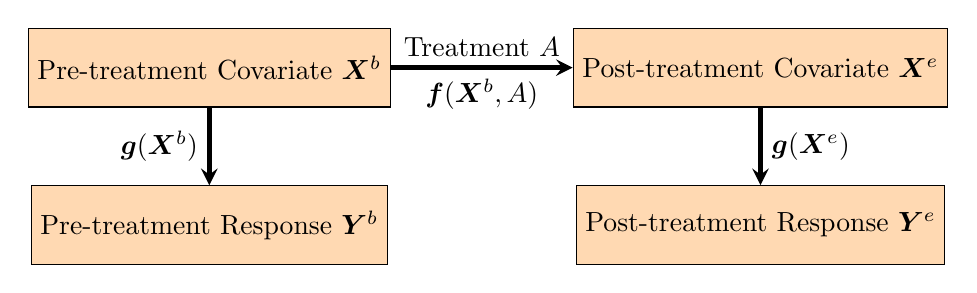
\begin{tikzpicture}[node distance=2cm]
    \tikzstyle{arrow} = [ultra thick,->,>=stealth]
    \node[rectangle, minimum width=3cm, minimum height=1cm, text centered, draw=black, fill=orange!30](PTX){Pre-treatment Covariate $\bm{X}^b$};
    \node[rectangle, minimum width=3cm, minimum height=1cm, text centered, draw=black, fill=orange!30, below of=PTX](PTY){Pre-treatment Response $\bm{Y}^b$};
    \node[rectangle, minimum width=3cm, minimum height=1cm, text centered, draw=black, fill=orange!30, 
    right of=PTX, xshift=5cm
    ](ATX){Post-treatment Covariate $\bm{X}^e$};
    \node[rectangle, minimum width=3cm, minimum height=1cm, text centered, draw=black, fill=orange!30, below of=ATX](ATY){Post-treatment Response $\bm{Y}^e$};
    \draw[arrow] (PTX)-- node[anchor=east]{$\bm g(\bm X^b)$} (PTY);
    \draw[arrow] (PTX)--node[anchor=south]{Treatment $A$} node[below] {$\bm f(\bm X^b, A)$}(ATX);
    \draw[arrow] (ATX)--node[anchor=west]{$\bm g(\bm X^e)$}(ATY);
    \end{tikzpicture}
    \caption{The data generating process. Both covariates $\bm X^b$ and responses $\bm Y^b$ are measured before a treatment, where responses are expressed through a postulated link function $\bm g(\bm X^b)$. Treatment $A$ affects covariates via the treatment effect function $f(\bm X^b, A)$, which yields post-treatment covariates $\bm X^e$. Post-treatment responses $\bm Y^e$ are generated with the same link function $\bm g(\bm X^e)$.}\label{fig1}
\end{figure}

This data generating process is visually presented in Figure \ref{fig1}. There are two unobserved functions: the treatment effect function $\bm f(\cdot)$ that alters the covariate values due to the treatment, and the link function $\bm g(\cdot)$ for the relationship between covariates and responses. More precisely, the treatment function $\bm f(\cdot)$ is defined as 
$$\bm f(\bm x,a) = E(\Delta \bm X | \bm X^b=\bm x,A=a).$$
Meanwhile, the link function between the covariate and the multivariate response (at either time point) is expressed as 
$$\bm g(\bm x) = E(\bm Y |  \bm X = \bm x).$$
Our goal of the estimation is the treatment effect, which can be intuitively understood as the difference of the potential outcomes \citep{rubin1974estimating} from the two treatments. However, this may not be easily modeled, especially when nonparametric structures are assumed. However, for a tree-based model, we may consider a simplified version at each internal node. 

\subsection{Modeling the treatment effects: internal node view}\label{Meth}

A tree-based method recursively slices the feature space, via binary splitting rules, such that the variation of the treatment effects of all outcomes within a node to be relatively small. However, given the complex form of the unknown treatment effect and link functions, it is difficult to construct such binary splits \citep{breiman2001random} in the form of $1(X^{j} > c)$ based on a single variable $j$. An oblique split \citep{menze2011oblique} can be more efficient, and we shall see that such techniques can be adapted to the multiple potential outcomes. 

Our proposed method works by locally approximate the within node data so that a splitting rule can be constructed. Note that this is not equivalent to making assumptions on the global model since recursive partitioning will serve as the main machinery to nonparametrically approximate the treatment effect function. At the internal node level, we may approximate $\bm f(\bm x,a)$ by assuming a linear function in the form of
$$\bm f(\bm x,a) = \bm f_0(x) + a \boldsymbol \beta_0 + a\bm B \bm x,$$
where $\bm f_0(x): \mathbb{R}^p \rightarrow \mathbb{R}^p$ is the averaged main effect, $\beta_0 \in \mathbb{R}^p$ and $\bm B \in \mathbb{R}^{p \times p}$ are coefficients for individual treatment effect. On the other hand, we could also approximate the link function $\bm g(\bm x)$ locally as 
$$\bm g(\bm x)= \bm \gamma_0 + \bm \Gamma \bm x,$$
where $\bm \gamma_0 \in \mathbb{R}^p$ is the intercept, and $\bm \Gamma \in \mathbb{R}^{q\times p}$ is a coefficient matrix. Under the above assumptions, the treatment effect can be modeled as
\begin{align}
    E(\Delta \bm Y | \bm X^b = \bm x, A = a) &= E(\bm Y^e | \bm X^b = \bm x, A = a)-E(\bm Y^b | \bm X^b = \bm x, A = a) \nonumber\\
    &=\bm \Gamma \left[E(\bm X^e | \bm X^b=\bm x, A = a) - E(\bm X^b | \bm X^b=\bm x,A = a)\right]\nonumber\\
    &=\bm \Gamma E(\Delta \bm X | \bm X^b=\bm x, A = a)\nonumber\\
    &=\bm \Gamma \bm f_0(x) +  a  \bm \Gamma \boldsymbol \beta_0 + a \bm \Gamma \bm B \bm x. \label{eqn:changeofy}
\end{align} 

Note that our parameter of interest is the treatment difference, which can be expressed as
\begin{align}
    \tau( \bm X^b = \bm{x}) &= E(\Delta \bm{Y}|\bm X^b = \bm x, A = 1) - E(\Delta \bm{Y}|\bm X^b = \bm x, A = -1) \nonumber \\
    &= 2 \bm \Gamma \boldsymbol \beta_0 + 2 \bm \Gamma \bm B \bm x. \label{eqn:treatmenteffect}
\end{align}

Instead of modeling $E(\Delta \bm{Y}|\bm X^b = \bm x, A = 1)$ for each treatment arm, which could be complicated, we borrow the modified outcome concept introduced in \cite{tian2014simple}, and model $\Delta \bm{Y} A$ as the outcome. This leads to
\begin{equation}
E(\Delta \bm Y A | \bm X^b = \bm x) = 2 \bm \Gamma \boldsymbol \beta_0 + 2 \bm \Gamma \bm B \bm x. \label{eqn:nodemodel}
\end{equation}

Without loss of generality, we may assume that the pre-intervention measures are centered, i.e., $E[\bm X^b] = 0$. Hence, with further centering of the outcome $\Delta \bm Y A$, the intercept term $2 \bm \Gamma \boldsymbol \beta_0$ can be removed. However, this formulation still cannot be directly used as the splitting rule since the outcome is still multivariate. However, we notice that if a linear combination is created using $\bm \alpha^T x$, while $\bm \alpha^T$ lies within the column space of $\bm \Gamma \bm B$, then splitting on $\bm \alpha^T x$ will effectively reduce the total variation of $\Delta \bm Y A$. Hence, the goal of our method is to construct such a split. Furthermore, the above equation does not use the information of $\bm X^e$ or $\Delta \bm X$. We shall show later that a three-way relationship can allow us to incorporate such information. Finally, we remark here that we may allow the link function $\bm g(x)$ to have time-specific constant $\bm \gamma_0$, which represent the potential change of confounding variables. This does not affect the formulation in the conditional expectation of $\Delta \bm Y$ in Equation \eqref{eqn:changeofy} except a constant change. Such a constant shall be removed for treatment effects in Equation \eqref{eqn:nodemodel} due to the randomness of treatment assignment. However, we may not allow the coefficient matrix to be different in the link function $\bm g(x)$.

\section{Multiple Outcome Treatment Effect Forests}\label{MOTE}
The core idea of our proposed method is a novel multivariate splitting rule that partition the feature space based on the estimated space of the individual treatment effect. The splitting rule takes the correlation structure of the multiple outcomes into consideration while utilizing the within node simplified model given in Equation \eqref{eqn:nodemodel}. Joint modeling of the changes in covariates and responses helps to constrain the searching space for splits. There are some attempts to extend the random forest framework to multivariate settings. \cite{Sega2011} replaced node impurity measure with a ``covariance" weighted analog. \cite{Rainforth2015} calculated impurity using projections of responses. But these extensions are not capable of modeling heterogeneity in the treatment effect. GUIDE \citep{Loh2015}, on the other hand, is a tree-based method that targets the individualized treatment effect and is compatible with multivariate response setting. However, GUIDE does not take advantage of repeated measures when analyzing the data. Hence, it is compelling to develop a device to model heterogeneity in treatment effects for multivariate outcomes while maximizing the efficiency of information utilization for pre- and post-intervention studies.

\subsection{MOTEF}
We are interested in locally estimating the difference of the post-treatment responses as described in Equation \eqref{eqn:treatmenteffect}. A random forest model is used to construct neighborhoods and perform the local averaging to predict treatment effects. The challenging part is to construct neighborhoods based on individualized treatment effect, implemented as splitting rules. The splitting rule construction is the core of the RF algorithm as it guides the model fitting process. When constructing the splitting rules, the change in impurity (variance reduction in regression random forests) associated with a split is quantified. The split that maximizes impurity change is selected. For the proposed method, we want to construct splitting rules so that each neighborhood contains nearly homogeneous subjects who experience similar treatment effects numerically defined in Equation \eqref{eqn:treatmenteffect}. 

Further exploring Equation \eqref{eqn:nodemodel}, we found that $\Delta \bm X A$ can also be modeled similarly. With proper centering to remove the intercept terms, we have
\begin{equation}
    E(\Delta \bm Y A | \bm X^b=\bm x) = \bm \Gamma E(\Delta \bm X A | \bm X^b = \bm x) = 2\bm \Gamma \bm B \bm x. \label{eqn:threesides}
\end{equation}

The interpretation of the above equation is as follows: The variations of the treatment effect $\Delta \bm Y A$ is contained within the linear subspace of $\bm X^b$ spanned by the column space of $\bm \Gamma \bm B$. In the meantime, the variations of the microbiome effect $\Delta \bm X A $ is contained within the linear subspace of $\bm X^b$ spanned by the column space of $\bm B$. The analysis of such multivariate data falls into the classic literature of canonical correlation analysis \citep{hotelling1936relations}, partial least squares \citep{wold2001pls}, and dimension reduction \citep{cook2010envelope}. However, instead of having two sets of variables in these classical settings, we now have three. These are referred to as multi-block models \citep{tenenhaus2011regularized, tenenhaus2017regularized} that draw attention in the integrative analysis of genetic data \citep{meng2016dimension, rohart2017mixomics} in recent years. By jointly model the signal across different sources, we may constrain the solution space of the splitting rule on $\bm X^b$. Here, we use a particular variation of the multi-block model, given by (as a population version):
\begin{align}
\{\bm{\widehat{\alpha}}, \bm{\widehat{\beta}}, \bm{\widehat{\kappa}}\} = & \argmax\limits_{\lVert\alpha\rVert^2 = \lVert\beta\rVert^2 = \lVert\kappa\rVert^2 = 1}
\Big[ \text{cov}( \bm \alpha\trnp \bm{X}^b, \bm \beta \trnp \Delta \bm{X} A ) + \nonumber \\ 
&\quad \text{cov} (\bm \alpha\trnp \bm{X}^b, \bm \kappa \trnp \Delta \bm{Y} A) +\text{cov}(\bm \beta\trnp \Delta \bm{X} A, \bm \kappa\trnp \Delta \bm{Y} A ) \Big] \label{eqn:multiblock}
\end{align}

The sample version of this optimization problem can be efficiently solved using spectral decomposition. Denote the ``up-right'' notations $\textbf{X}^b_{n \times p}$, $(\Delta \textbf{X}A)_{n \times p}$, and $(\Delta \textbf{Y}A)_{n \times q}$ as the observed data matrices. Without loss of generality, we assume that they are already properly centered column-wise. Then, we construct two augmented matrix as follows
\begin{align*}
\textbf{L} = \begin{pmatrix}
\textbf{X}^* & \textbf{0} & \textbf{0} \\
\textbf{0} & \textbf{0} &\Delta \textbf{Y}^*\\
\textbf{0} & \Delta \textbf{X}^*& \textbf{0}\\
\end{pmatrix},
\qquad
\textbf{R} = \begin{pmatrix}
\textbf{0} & \Delta \textbf{X}^* & \textbf{0}\\
\textbf{X}^* & \textbf{0} & \textbf{0} \\
\textbf{0} & \textbf{0} &\Delta \textbf{Y}^*\\
\end{pmatrix}.
\end{align*}
It can be easily seen that if we concatenate the three vectors $\alpha$, $\beta$ and $\kappa$ as $\bm{v} = (\alpha^T, \beta^T, \kappa^T)^T$ and remove the individual norm constraints, then the objective function defined in Equation \eqref{eqn:multiblock} can be written into
\begin{align}
\widehat{\bm{v}} = \argmax\limits_{\lVert\bm{v}\rVert^2 = 1} \quad \bm{v}^T \textbf{L}^T \textbf{R} \bm{v}
= \argmax\limits_{\lVert\bm{v}\rVert^2 = 1} \quad \frac{1}{2} \bm{v}^T (\textbf{L}^T \textbf{R} + \textbf{R}^T \textbf{L}) \bm{v},
\end{align}
which can be solved by performing singular-value decomposition of the augmented symmetric matrix $\textbf{L}^T \textbf{R} + \textbf{R}^T \textbf{L}$. Note that the constraints on the original three loading vectors does not play a role since the corresponding columns in both $\textbf{L}$ and $\textbf{R}$ are block-wise orthogonal. Hence the corresponding blocks in $\bm{v}$ will be proportional to each of the three loading vectors, respectively. Note that there is relatively dense literature on different formulations of multi-block or multi-way canonical correlation analysis and our formulation is only a specific choice. For this topic, we refer to \cite{tenenhaus2017regularized}. Nonetheless, we believe that using the covariance formulation instead of correlation is more sensible because the splitting rules can then be performed in the direction with large variations. This leads to the advantage that the heterogeneity of treatment effects at each terminal node is relatively small. 

After recovering $\widehat \alpha$, $\widehat \beta$ and $\widehat \kappa$ from $\widehat{\bm{v}}$, it is natural to use the estimated linear combination of pre-treatment covariates, $\bm{\hat{\alpha}}\trnp \bm X^b$, as the variable to partition the local population. Then we could find the best split that maximizes the impurity reduction in terms of the outcome $\kappa\trnp \Delta \bm{Y}A$. Here, the impurity of a node $\cal N$ is simply the sample variance of $\Delta \bm{Y} A$ within the node:
\[
    \text{Impurity}({\cal N})  = \frac{1}{|\cal N|}\sum_{i \in {\cal N}} \left(\bm{\widehat{\kappa}}\trnp \Delta \bm{Y}_i \cdot A_i - \frac{1}{|\cal N|}\sum_{i \in \cal N} \bm{\widehat{\kappa}}\trnp \Delta \bm{Y}_i \cdot A_i\right)^2,
\]
where $|{\cal N}|$ denotes the sample size within node ${\cal N}$. Our split is constructed based on linear combinations of the pre-intervention covariates $\bm{X}^b$ while the best splitting point is selected by searching for the best split that reduces the combined impurity of both potential child nodes. Alternatively, random splitting points \citep{geurts2006extremely} can also be considered. When predicting, MOTEF requires only pre-treatment covariates $\bm{X}^b$, and returns the within node average of $\Delta \bm{Y} A$, which is the estimated treatment differences defined in Equation \eqref{eqn:treatmenteffect}. A pseudo algorithm is provided in Algorithm \ref{alg:rf}.

\begin{algorithm}
    \caption{Pseudo algorithm for \textproc{MOTEF}}
    \begin{algorithmic}[1]
        \INPUT training data ${\cal D}_n = \{\bm X^b_i, \bm Y^b_i, A_i, \bm X^e_i, \bm Y^e_i\}_{i=1}^n$, number of random splits $\texttt{nsplits}$
        \OUTPUT an ensemble tree model
        \STATE For each tree, at an internal node ${\cal N}$, stop if the sample size is sufficiently small
        \STATE Conduct augmented optimization to solve for $\widehat \alpha$, $\widehat \beta$ and $\widehat \kappa$.
        \STATE Randomly generate $\texttt{nsplits}$ cutting points from the fist canonical projection, $\bm{\hat{\alpha}}\trnp \bm X^b$ 
        \STATE For each candidate split, denote ${\cal N}_L$ and ${\cal N}_R$ as the two child nodes resulting from the candidate split. Calculate the change in impurity:
        \[
        \text{score}( {\cal N}_L, {\cal N}_R) = |{\cal N}_L| \text{Impurity}({\cal N}_L) + |{\cal N}_R|\text{Impurity}({\cal N}_R).
        \]
        \STATE Select the candidate split with the minimum score, and apply 1-4 to each child node.
        \STATE Repeat 1-5 for each tree until the desired number of trees are fitted.
    \end{algorithmic} \label{alg:rf}
\end{algorithm}

\section{Numeric Studies}\label{Sim}

We use synthetic data to investigate the performance of the proposed method. Due to the limited literature for multivariate outcomes in the precision medicine setting, we compare our approach with two new approaches. The first approach simply extends the penalized least square estimator of \citep{qian2011performance} to a multivariate case by using the multivariate Gaussian family model implemented in the \texttt{glment} 3.0-2 package \citep{glmnet}. The second approach fits a univariate random forest model to each component of the outcome. This is carried out using the \texttt{randomForest} 4.6-14 package \citep{liaw2002classification}. We consider six different settings following the data generating process below:
\begin{enumerate}
    \item Generate $\bm{X}^b$ from a multivariate Gaussian distribution, MVN($\bm 0$, $\bm \Sigma_{p \times p}$).
    \item Generate the treatment label independent from a binomial distribution, $A \sim$ Bern(0.5), and generate the post-treatment covariate $\bm X^e$ via the treatment effect function $\bm f(\cdot)$
    \[
        \bm{X}^e = \bm{X}^b + \bm f(\textbf{X}^b, \text{A}) + \textbf{e}_x, \quad \textbf{e}_x \sim \text{MVN}(\bm 0, \sqrt{3}^{-1} \bm I_{p \times p})
    \]
    \item Generate the pre- and post-treatment responses $\bm{Y}^b$ and $\bm{Y}^e$ via the link function $\bm g(\cdot)$
    \[
        \bm{Y} = \bm g(\bm{X}) + \textbf{e}_y, \quad \textbf{e}_y \sim \text{MVN}(\bm 0, \sqrt{3}^{-1} \bm I_{q \times q})
    \]
\end{enumerate}

We consider both linear and nonlinear functions of $\bm f(\textbf{x}, a)$ and $\bm g(\textbf{x})$. In settings 1 - 3, $\bm \Sigma = \bm I$, and for settings 4 - 6, $\bm \Sigma_{ij} = 0.8^{|i-j|}$. For settings 1, 2, 4, 5, we use linear treatment effect functions where $\bm f(\textbf{x}, a) = a\textbf{B}\textbf{x}$, while for the other two settings, $\bm f(\textbf{x}, a) = a(\textbf{B}\textbf{x})^2$. For the link function $\bm g(\textbf{x})$, we use a linear model $\bm g(\textbf{y}) = \bm \Gamma\textbf{y}$ for settings 1, 3, 4 and 6, and use $\bm g(\textbf{y}) = \bm \Gamma\textbf{y}^2$ for the rest. Note here that the square operation is element-wise. The coefficient matrices $\bm{B}_{10 \times 10}$ is designed such that the upper-left block equals $\sqrt{3}^{-1} [ \mathbf{I}_{3 \times 3}  \otimes (1,2,3)^T, \mathbf{I}_{3 \times 3} \otimes (1,-2,-3)^T, \mathbf{I}_{3 \times 3} \otimes (1,-2,3)^T ]$, and the rest of the elements are filled with 0. The $\bm \Gamma$ matrix is given by 
$$
  \bm \Gamma = \frac{1}{\sqrt{7}}
  \begin{pmatrix}{}
  1 & 2 & 3 & 0 & 0 & 0 & 0 & 0 & 0 \\
  0 & 0 & 0 & -1 & -2 & -3 & 0 & 0 & 0 \\
  0 & 0 & 0 & 0 & 0 & 0 & 1 & -2 & 3 \\
  \end{pmatrix}^T.
$$
The blocked structure in both $\bm B$ and $\bm \Gamma$ will automatically impose a correlation structure on the multivariate outcomes. We use $p=10$ and $q = 3$ in all simulation settings. We use 400 training samples and 1000 testing samples in each setting. For penalized linear regression ($l_1$-PLS), we use the 10-fold cross-validation implemented in the \texttt{glmnet} package. For the marginal random forest method, the default tuning is used. For the proposed method, we set the number of trees to be 200, and use random splitting rules with 10 randomly generated cutting points at each node \citep{geurts2006extremely}. To evaluate the performance, we calculate the marginal mean squared error (MSE) of the estimated treatment effects across 200 iterations of the simulations and aggregate the errors overall outcome dimensions. All computation was conducted on a high-performance 64-bit Linux platform with 48 cores of 2.70GHz eight-core Intel Xeon E5-2680 processors with 24G of RAM per core and R 3.6.0 \citep{R2020}. All model fitting was run using a single core.

\subsection{Simulation Result}\label{3.2}
Simulation results are shown in Table \ref{SimRes}. Overall, models constructed using the proposed MOTEF have smaller aggregated prediction error than competing methods in nonlinear settings, i.e., either the treatment effect function or the link function is nonlinear. When both functions are linear, $l_1$-PLS model inevitably performs better (MSE = 0.21) than MOTEF (0.83) and Marginal RF (1.43). The advantage of using MOTEF is substantial when either function is nonlinear. When $f$ is linear and $g$ is polynomial, the MSE of MOTEF is 72\% and 88\% of the MSE from $l_1$-PLS and marginal RF, respectively. The discrepancy in performance is more obvious when the correlation structure exists in pre-treatment covariates. This is consistent with our splitting rule construction, which is intended to utilize the correlation structure among the multiple outcomes. Overall, the proposed MOTEF has 66\% and 87\% error compared with marginal RF when either of $\bm f$ and $\bm g$ is non-linear. And the advantage over the linear models is more significant. Computation wise, it takes, on average, less than 1 minute to fit the proposed model for the simulated datasets. 
%cost are documented in Table \ref{CompRes}. The proposed method requires longer time and larger space to fit and store the model compared to the $l_1$-PLS and marginal RF. As the dimensional of the data increase, the advantage on storage size of Marginal RF over the proposed model MOTEF gradually shrinks. Overall, even though the proposed method takes longer time to fit, the computation time and required space is acceptable. The proposed method is feasible to use on a modern computer.


\section{Real Data Analysis}\label{realdata}
We applied the proposed method to analyze two recent food and nutrition studies, almond consumption study by \citet{holscher2018almond} and avocado consumption study by \citet{Avocado}. Both studies were interested in examining how food consumption affects the composition of the gastrointestinal microbiota and host characteristics. 

For both studies, we fitted a MOTEF model containing 200 trees. Considering the limited sample sizes, we selected 15 operational taxonomic units (OTUs) at the genus level as covariates, where the OTU selection follows the same workflow. All genus-level OTUs were firstly filtered by their prevalence according to \cite{callahan2016bioconductor}, where the relative abundance of an OTU across all samples should be greater than 1e-5, and the OTU should present in 80\% of all sample. Screening using Wilcox's Rank Sum test between the two treatment groups is used afterward. The top 15 OTUs with the smallest p-values were selected as covariates in our MOTEF model. As mentioned in Section \ref{Notation}, microbiome data are compositional. Hence, the log-ratio transformation was applied to the OTUs, where the sum of abundances of the unselected OTUs are used as the denominator. Mathematically, the transformed abundance $x_{ij}^*$ is
\begin{equation*}
    x_{ij}^* = \log\Big(\frac{x_{ij}}{\sum\limits_{o \in O} x_{io}}\Big),    
\end{equation*}
where $x_{ij}$ is the relative abundance for $j$th OTU from the $i$th participants,
$O$ is the index set of OTUs that are not selected as the covariates. Due to the high sparsity of this dataset, a small number (1e-11) was added to the relative abundance to prevent infinite value during the transformation. Outcomes of the studies were standardized before the model fitting. Demographic variables are used as confounding in the analyses: sex, age at baseline, and body mass index at baseline in the almond consumption analysis, and body mass index at baseline in the avocado consumption analysis. To accommodate the confounding demographic variables in the algorithm, we modified Equation \eqref{eqn:multiblock} as the following:
\begin{align}
\{\bm{\widehat{\alpha}}, \bm{\widehat{\beta}}, \bm{\widehat{\kappa}}\} = & \argmax\limits_{\lVert\alpha\rVert^2 = \lVert\beta\rVert^2 = \lVert\kappa\rVert^2 = 1}
\Big[ \text{cov}( \bm \alpha\trnp \left[ \bm Z : \bm{X}^b\right], \bm \beta \trnp \Delta \bm{X} A ) + \nonumber \\ 
&\quad \text{cov} (\bm \alpha\trnp \left[ \bm Z : \bm{X}^b\right], \bm \kappa \trnp \Delta \bm{Y} A) +\text{cov}(\bm \beta\trnp \Delta \bm{X} A, \bm \kappa\trnp \Delta \bm{Y} A ) \Big], \label{eqn:multiblock2}
\end{align}
where $\bm Z$ is a random vector containing the demographic variables and $\left[\bm Z:\bm X^b\right]$ denotes the concatenation of the two vectors.

Given the MOTEF model, out-of-bag predictions of individualized treatment effects were made and visually presented in Spaghetti plots. We further investigated the effect of microbiota on the individualized treatment effect. Due to the ``black box" nature of random forest algorithms \citep{breiman2001statistical}, we used feature importance to identify relevant OTUs without giving directional inference. Feature importance is calculated by decomposing an estimation matrix of the outer products of oblique splits weighted by sample size and aggregated over all trees. Precisely, the estimation matrix is
\begin{equation*}
    \widehat{M} = \sum\limits_{{\cal T} \in {\cal F}} \sum\limits_{{\cal N} \in {\cal T}}|{\cal N}|\bm \alpha_{\cal N} \bm\alpha_{\cal N}\trnp,
\end{equation*}
where $\bm \alpha_{\cal N}$ is the splitting direction at the internal node ${\cal N}$ of the tree ${\cal T}$ in the forest. $|\cdot|$ denotes the sample size of the node. Note that when the assumed linear model is true and without noise, all $\alpha_{\cal N}$ are also contained in the column space of $\bm \Gamma \bm B$. Hence, the eigenvectors of the estimation matrix $\widehat{M}$ will also be contained within the same column space. Finally, the importance of OTUs is calculated by summing the absolute value of all eigenvectors scaled by the corresponding eigenvalue of $\widehat{M}$. This is motivated by the estimation matrix construction in the dimension reduction literature \citep{li1991sliced}.

\subsection{Almond Consumption Data}
The almond data set was collected in a recent study \citep{holscher2018almond} that examined how almond consumption affects the composition of the gastrointestinal microbiota and host characteristics. Participants of the study were randomly assigned to 5 diets: control, almond butter, chopped almonds, whole roasted almonds, and whole natural almonds. We combine the control and almond butter groups as the ``control'' group because almond butter is too easy for the human digestive system to process and do not effectively promote gut microbiota growth. Hence almond butter works similarly to the control. Chopped and whole roasted almonds are grouped as the ``treatment'' group. In the data set, we had a total of 68 subjects, 32 in the almond group and 36 in the control group. The biomarkers measured in the study included interleukin-6 (IL6), C-reactive protein (CRP), serum amyloid A (SAA), soluble intercellular adhesion molecules (SICAM1, SVCAM1).

The predicted individual treatment effects are presented in Figure \ref{AlmondPlot} in a spaghetti plot. Each line represents the predicted treatment effect of the biomarkers from one study participant. We further apply a K-mean clustering algorithm on the predicted multivariate treatment effect, where 3 clusters are created. Overall, the change of CRP and IL6 would have a modest difference between the "control" diet and the almond diet. The unresponsiveness of CRP and IL6 coincides with the observation in another fruit and vegetable intake study \citep{nadeem2014serum}. Nevertheless, individuals still experience treatment effects differently. For example, comparing the almond diet to the ``control'' diet, individuals in cluster 1  are more sensitive to SICAM1 change and less sensitive to SAA change, while the opposite is true for individuals in Cluster 3. Meanwhile, the heterogeneity in treatment effect also reflects in CRP and IL6. While the individuals in Cluster 3 would have higher CRP and IL6 values if they took almond diet instead of ``control'' diet, the individuals in Cluster 2 would have lower values. Moreover, via the feature importance presented in  Table \ref{AlmondFI}, we identified important OTUs at the genus level are an unclassified genus level OTU in the \textit{Lachnospiraceae} family, \textit{Blautia}, and \textit{Ruminococcus}. Previous literature shows that \textit{Blautia} is linked to visceral fat area \citep{ozato2019blautia} and \textit{Ruminococcus} may be vital to plant cell wall breakdown in the human colon \citep{ze2012ruminococcus}.

\subsection{Avocado Consumption Data}
The avocado data set comes from another diet trial \citep{Avocado} that examines the effects of avocado consumption on the intestinal microbiota and metabolic health. Participants of the study were randomly assigned to two diet interventions (avocado diet and control diet) on a 1:1 ratio. Gastrointestinal microbiota and host biomarkers were measured before and after the 12-week intervention period. Only complete cases were used in the data analysis, where there were 54 participants in each treatment group. The biomarkers were standardized diastolic blood pressure (DBP), systolic blood pressure (SBP), LDL-cholesterol, and Triglycerides (TG).

The predicted individual treatment effects are presented in Figure \ref{AvocadoPlot} in a spaghetti plot. We further apply a K-mean clustering algorithm on the predicted multivariate treatment effect, where 3 clusters are created. We found great heterogeneity in the treatment effect. For individuals in Cluster 1, consuming either treatment (avocado or control) would yield similar benefits. For individuals in cluster 3, consuming avocado would have lower SBP and TG than consuming control, but would not necessarily help as much for lowering LDL. In constrast, individuals in Cluster 2 would not have lower SBP and TG, if not increase, than consuming control. Using feature importance visually presented in Table \ref{AvocadoFI}, the top three important OTUs are the unclassified OTU at genus level from \textit{Lachnospiraceae} family, \textit{Ruminococcus}, and \textit{Roseburia}. In previous literature, \textit{Roseburia} has been found to be associated with weight loss and glucose tolerance \citep{ryan2014fxr}, and \textit{Ruminococcus} may be vital to plant cell wall breakdown in the human colon \citep{ze2012ruminococcus}.


\section{Discussion}\label{Disc}

In this paper, we propose a random forest framework to model the heterogeneous treatment effects when the outcome is multivariate. The essential idea is to partition the feature space based on linear combinations of the covariates, while the loading vector is learned based on a local linear approximation of the treatment effect function at each internal node. Furthermore, our method addresses a challenge in the complete feeding study design where microbiota is measured both before and after the food intervention. Overall, the contribution of the proposed method is three-fold: 1) it brings a new possibility for simultaneous modeling of multiple bio-markers with full consideration of the covariance structures among predictors and outcomes; 2) the model is extremely flexible to model nonlinear signals, and 3) it maximizes the utilization of collected information to improve the accuracy of prediction. 

Even though the proposed method's primary purpose is to model the treatment effect, many extensions could be easily accomplished, including treatment recommendation and subgroup analysis. The treatment recommendation is always based on a reward function of treatments \citep{qian2011performance}. The reward function is well-defined when the outcome is univariate. Nevertheless, defining the reward function for a multivariate outcome is non-trivial, especially when lacking domain knowledge. However, given a direction where the improvement would be expected to happen, the better treatment could be decided by simply projecting the predicted individual treatment effect on the given direction. On the other hand, subgroup analysis is also possible via a MOTEF model. Given the random forest kernel proposed by \cite{davies2014random}, the distance of samples can be calculated. A clustering step would yield similarity groups, which can be used to learn the underlying subgroups.

The proposed model also has disadvantages. In our derivation, we require a randomized trial, which is slightly restrictive. However, this restriction can be lifted by adopting sampling weights. \cite{tian2014simple} provided theoretical justification for using the probability of treatment allocation as weights during model fitting. Secondly, the current implementation focuses on cases where covariates are time-sensitive, not directly applicable to studies that include time-invariant covariates, such as sex or race. A simple modification is to add the time-invariant variables in the pre-treatment covariate matrix $\textbf{X}^b$, but not in the difference matrix of covariate $\Delta \textbf{X}$. Thirdly, under high dimensional settings, the proposed loading estimations via the CCA could be numerically unstable in the lower level internal nodes, as the sample size is relevantly close to or smaller than the number of covariate or response dimensions. This forces the algorithm to stop, and would be detrimental to the accuracy of the prediction. We expect a regularized CCA algorithm to be able to address this. However, the computational cost might be greatly increased. %\bg{Lastly, the model assumption requires the before and post treatment link functions to be the same so that the borrowed information from post-treatment covariates can be used to regularize the solution space of CCA. This can be generalized to the degree that the two link functions differ by an constant term, for example, $g^b(x) = g(x)$ and $g^e(x) = g(x) + c$ for a constant $c$. Nevertheless, when the two functions are completely different, the improvement in treatment effect prediction are not studied yet. }

Future efforts will be spent on specializing the method for high-resolution microbiome data analysis. Microbiome data are usually high-dimensional by nature. Analyzing high-resolution microbiome data would require a larger sample size under the current framework. Meanwhile, signals for OTUs are generally small, which would induce inefficient splits. Grouping weak effects using external biological information, such as a phylogenetic tree, could increase the power of detecting real associations \citep{peterson2016joint}, hence improving prediction accuracy. Incorporating the biological information into the joint modeling of the microbiome and outcomes in the CCA step would be a promising solution, where \citet{chen2013structure} would provide a helpful reference. 

% \section*{Declarations}
% \section*{Funding}
% \section*{Conflicts of interest}
% \section*{Availability of data and material}
% Not applicable.
\section*{Code availability }
The method has been implemented in a freely available R package MOTE.RF at \url{https://github.com/boyiguo1/MOTE.RF}.


% Discussion of using repetitive measusres
% As the price of data storage is close to negligible, it is a normal practice to collect data repeatedly over time. Different modelling strategies of the repeatedly measured data can easily lead to different estimations. Cross-sectional models produce different results from what longitudinal models produce. Hence, interpreting cross-sectional models in a longitudinal fashion will lead to a big problem. How to effectively model repeatedly measured data is of big concern, especially for precision medicine research.

% Discussion of Interpretation
% Interpretation for random forest models is difficult. Feature importance is a commonly used tool to interpret the predictors for random forest. In this article, we provided a feature importance algorithm, demonstrated with the almond assumption data.

\clearpage


\begin{table}[h]
    \centering
    \begin{tabular}{l l l c c c c}
    \hline
    & &    &\multicolumn{3}{@{}c@{}}{\textbf{Independent}} \\
    \cmidrule(lr){4-6}
    Setting & $f(x)$ & $g(x)$ & MOTEF & $l_1$-PLS & Marginal RF\\
    \hline
    1 & Linear & Linear & 0.83 (0.13) & 0.21 (0.05) & 1.43 (0.12)\\
    2 & Linear & Polynomial & 16.87 (1.67) & 23.32 (1.54) & 19.01 (1.58)\\
    3 & Polynomial & Linear & 42.99 (3.87) & 43.62 (3.01) & 59.74 (4.19)\\
    \hline
    & &    &\multicolumn{3}{@{}c@{}}{\textbf{Correlated}} \\
    \cmidrule(lr){4-6}
    Setting & $f(x)$ & $g(x)$ & MOTEF & $l_1$-PLS & Marginal RF\\
    \hline
    4 & Linear & Linear & 0.80 (0.10) & 0.20 (0.05) & 0.82 (0.1)\\
    5 & Linear & Polynomial & 20.50 (3.72) & 52.73 (6.06) & 31.07 (4.81)\\
    6 & Polynomial & Linear & 35.26 (6.59) & 129.12 (15.33) & 40.61 (7.10)\\
    \hline
    \end{tabular}                  
    \caption{Mean (SD) of aggregated prediction error of treatment effect.}\label{SimRes}
\end{table}


%%%%%%%%% Original Table One: correponding to R implementation of MOTE RF %%%%%%%%%%%%%%%%%%%%%%%%
%\begin{table}[h]
%    \centering
%    \begin{tabular}{l l l c c c c}
%    \hline
%    & &    &\multicolumn{3}{@{}c@{}}{\textbf{Independent}} \\
%    \cmidrule(lr){4-6}
%    Setting & $f(x)$ & $g(x)$ & MOTEF & $l_1$-PLS & Marginal RF\\
%    \hline
%    1 & Linear & Linear & 0.93 (0.12) & 0.21 (0.05) & 1.42 (0.12) \\
%    2 & Linear & Polynomial & 15.62 (1.56) & 23.26 (1.52) & 19.02 (1.51)\\
%    3 & Polynomial & Linear & 37.5 (3.27) & 43.65 (3.02) & 59.77 (4.13)\\
%    \hline
%    & &    &\multicolumn{3}{@{}c@{}}{\textbf{Correlated}} \\
%    \cmidrule(lr){4-6}
%    Setting & $f(x)$ & $g(x)$ & MOTEF & $l_1$-PLS & Marginal RF\\
%    \hline
%    4 & Linear & Linear & 0.89 (0.11) & 0.2 (0.05) & 0.82 (0.1)\\
%    5 & Linear & Polynomial & 17.31 (3.33) & 53.03 (6.04) & 31.24 (4.77)\\
%    6 & Polynomial & Linear & 33.18 (7.19) & 130.52 (15.17) & 41.03 (7.44)\\
%    \hline
%    \end{tabular}                  
%    \caption{Mean (SD) of aggregated prediction error of treatment effect.}\label{SimRes}
%\end{table}





%%%%%%% Computation Cost Table %%%%%%%%%%%%%%%%%%%%%%%
%\begin{table}[h]
%    \centering
%\begin{tabular}{l l c c c c c c}
%\hline
%    & & \multicolumn{3}{@{}c@{}}{\textbf{Time (in seconds)}} & \multicolumn{3}{@{}c@{}}{\textbf{Size (in kilobytes)}}\\
%    \cmidrule(lr){3-5}\cmidrule(lr){6-8}
%p & q  & MOTEF & $l_1$-PLS  & Marginal RF & MOTEF &  $l_1$-PLS  & Marginal RF\\
%\hline
%10 & 3 & 50.103 & 0.006 & 0.879 & 32304.16 & 15.300 & 5669.32\\
%20 & 6 & 74.155 & 0.010 & 3.363 & 19606.92 & 35.526 & 11238.22\\
%\hline
%\end{tabular}
%   \caption{Mean computation time in seconds and object size in kilobytes, averaging over 200 iterations of 6 aforementioned simulation settings with different variable sizes.  For the proposed method, we set the number of trees to be 200, and use random splitting rules with 10 randomly generated cutting points at each node.For penalized linear regression ($l1$-PLS), we use the 10-fold cross-validation implemented in the \texttt{glmnet} package. For the marginal random forest method, the default tuning parameters in \texttt{randomForest} package are used.}\label{CompRes}
%\end{table}

\begin{figure}[h]
    \centering
    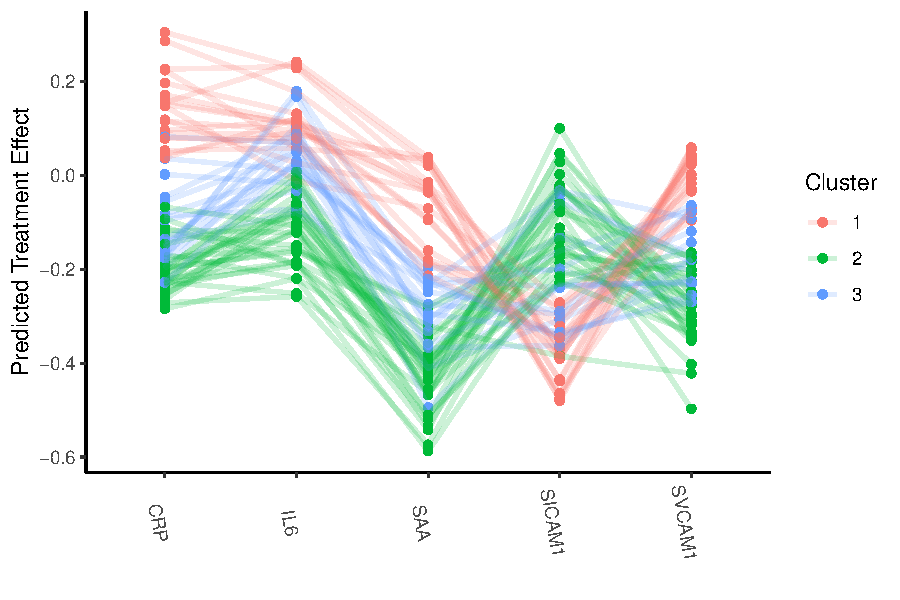
\includegraphics[width = %\textwidth]{Fig2_AlmondTreatmentEffect_V2.pdf}
    \textwidth]{Figures/Fig2_AlmondTreatmentEffect_V3.pdf}
    \caption{ Out of bag prediction of individualized treatment effect comparing almond diet to control diet. The serum inflammatory markers, including interleukin 6 level (IL6), C-reactive protein (CRP), serum amyloid A (SAA), soluble intercellular adhesion molecules (SICAM1, SVCAM1), are standardized. Each line represents an individual. K-mean clustering algorithm is applied to the predicted treatment effect of the 5 biomarkers, and generate 3 groups whose treatment effects of the five-dimensional outcome are similar within.}\label{AlmondPlot}
\end{figure}



%\begin{figure}[h]
%    \centering
%    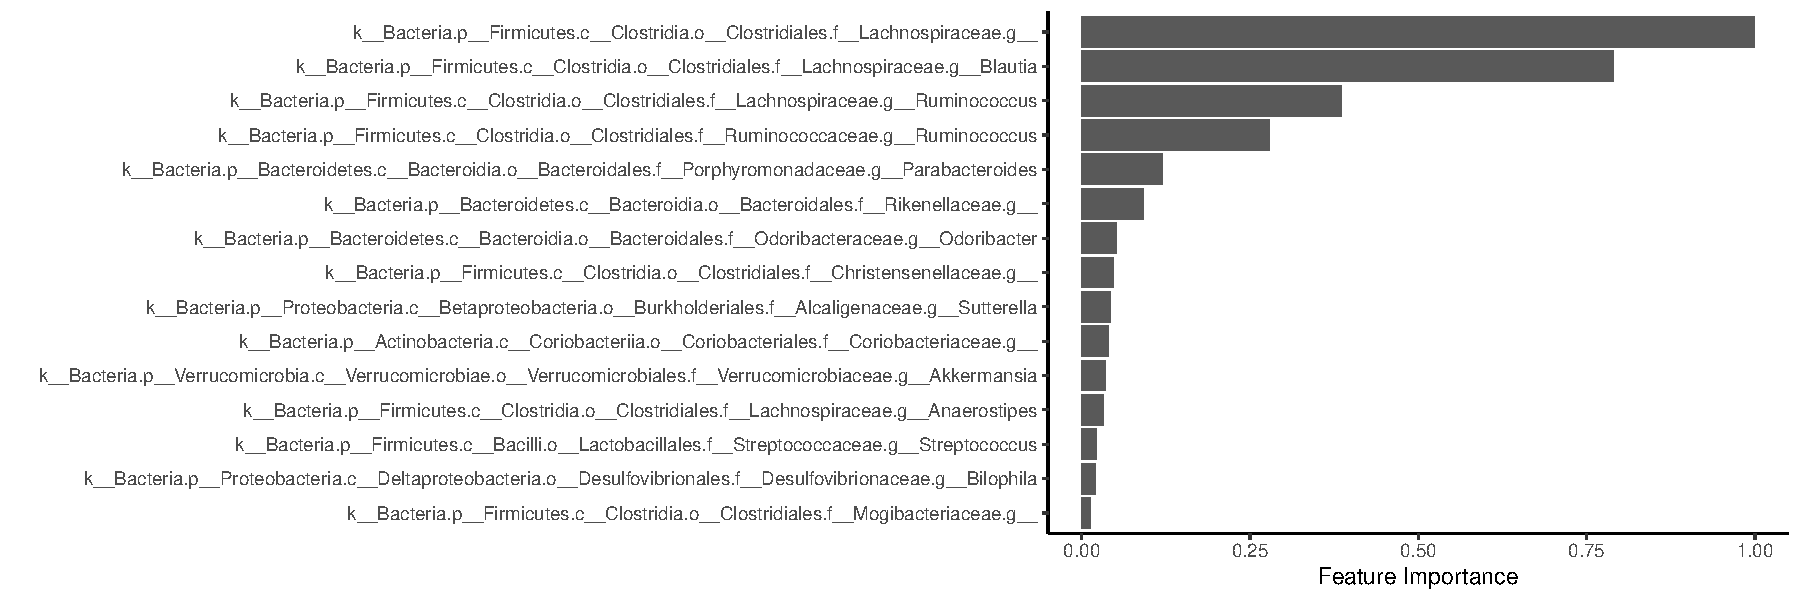
\includegraphics[width = \textwidth]{Fig3_AlmondFI.pdf}
%    \caption{Feature importance of the operational taxonomic units at the genus level in the almond consumption data analysis}\label{AlmondFI}
%\end{figure}


\begin{table}[h]
    \centering
\begin{tabular}{l l l l c}
\hline
Class & Order & Family & Genus & Relative\_Importance\\
\hline
Clostridia & Clostridiales & Lachnospiraceae & unclassified & 0.63\\
Clostridia & Clostridiales & Lachnospiraceae & Blautia & 0.44\\
Clostridia & Clostridiales & Ruminococcaceae & Ruminococcus & 0.40\\
Bacteroidia & Bacteroidales & Rikenellaceae & unclassified & 0.36\\
Clostridia & Clostridiales & Lachnospiraceae & Ruminococcus & 0.17\\
\hline
\end{tabular}
\caption{The top 5 important genera in the almond consumption data analysis. All of the top 5 important genera belong to the bacteria kingdom and the firmicutes phylum.}\label{AlmondFI}
\end{table}

%\begin{table}[h]
%    \centering
%\begin{tabular}{l l l l l c}
%\hline
%Phylum & Class & Order & Family & Genus & Relative\_Importance\\
%\hline
% Firmicutes & Clostridia & Clostridiales & Lachnospiraceae & unclassified & 1.00\\
% Firmicutes & Clostridia & Clostridiales & Lachnospiraceae & Blautia & 0.78\\
% Firmicutes & Clostridia & Clostridiales & Lachnospiraceae & Ruminococcus & 0.37\\
% Firmicutes & Clostridia & Clostridiales & Ruminococcaceae & Ruminococcus & 0.26\\
% Bacteroidetes & Bacteroidia & Bacteroidales & Porphyromonadaceae & Parabacteroides & 0.13\\
%\hline
%\end{tabular}
%\caption{The top 5 important genera in the almond consumption data analysis. All genera belong to the bacteria kingdom.}\label{AlmondFI}
%\end{table}


\begin{figure}[h]
    \centering
   % 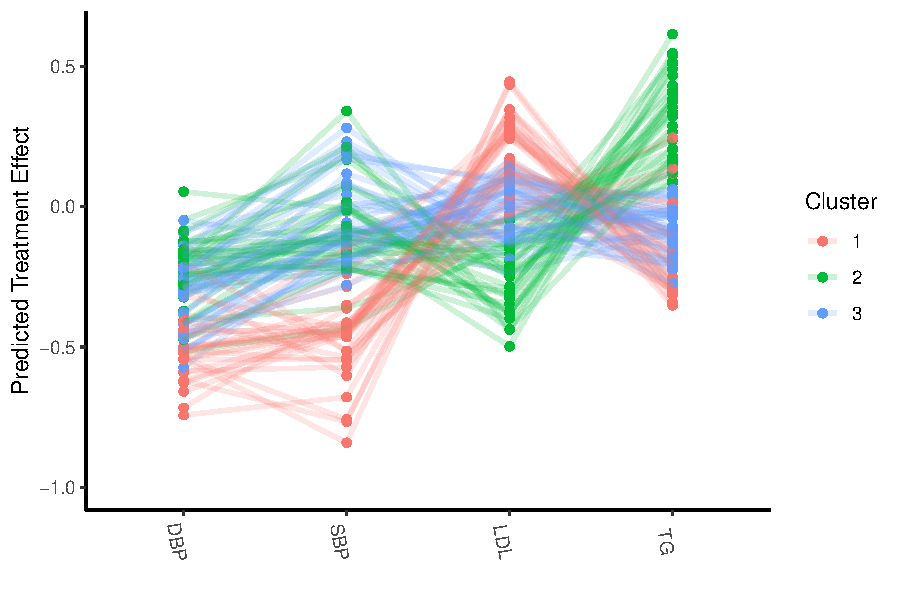
\includegraphics[width = \textwidth]{Fig4_AvocadoTreatmentEffect_V2.pdf}
    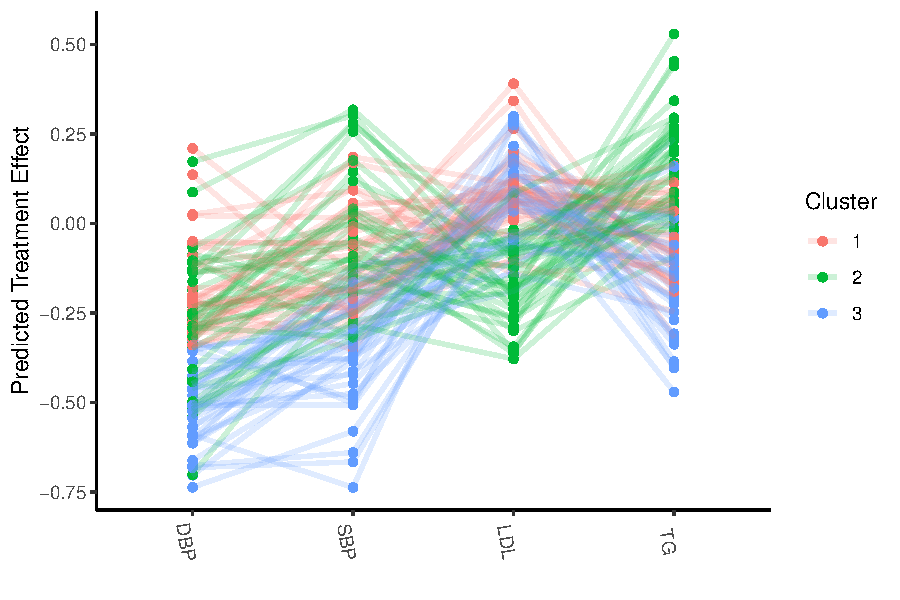
\includegraphics[width = \textwidth]{Figures/Fig4_AvocadoTreatmentEffect_V3.pdf}
    \caption{ Out of bag prediction of individualized treatment effect comparing avocado diet to control diet. The biomarkers, including diastolic blood pressure (DBP), systolic blood pressure (SBP), low-density lipoproteins cholesterol (LDL), and triglycerides (TG), are standardized. Each line represents an individual. K-mean clustering algorithm is applied to the predicted treatment effect of the 5 biomarkers, and generate 3 groups whose treatment effects of the five-dimensional outcome are similar within.}\label{AvocadoPlot}
\end{figure}


%\begin{figure}[h]
%    \centering
%    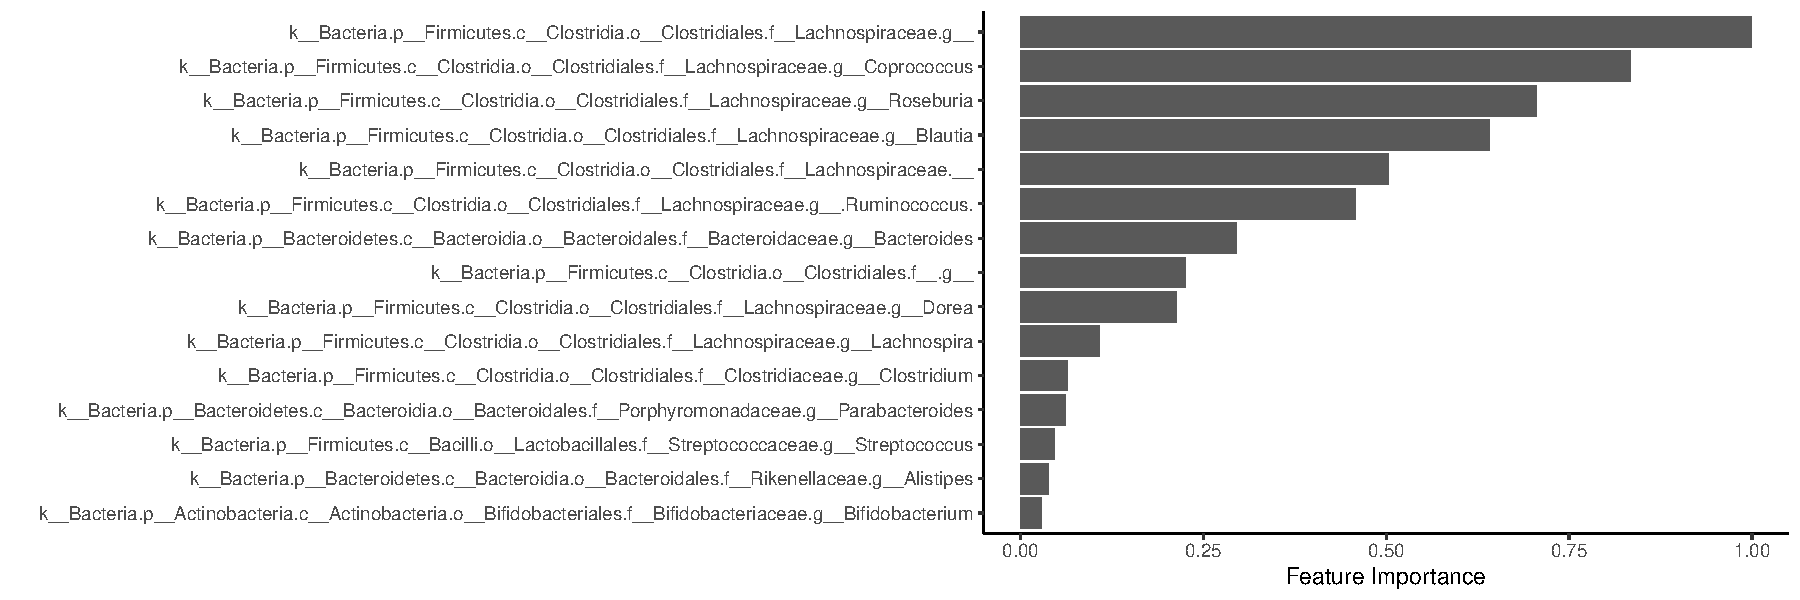
\includegraphics[width = \textwidth]{Fig5_AvocadoFI.pdf}
%    \caption{Feature importance of the operational taxonomic units at the genus level in the avocado consumption data analysis}\label{AvocadoFI}
%\end{figure}

\begin{table}[h]
    \centering
\begin{tabular}{l l l l c}
\hline
Class & Order & Family & Genus & value\\
\hline
Clostridia & Clostridiales & Lachnospiraceae & unclassified & 1.00\\
Clostridia & Clostridiales & Lachnospiraceae & Ruminococcus & 0.46\\
Clostridia & Clostridiales & Lachnospiraceae & Roseburia & 0.35\\
Clostridia & Clostridiales & Lachnospiraceae & Dorea & 0.35\\
Clostridia & Clostridiales & Lachnospiraceae & Blautia & 0.27\\
\hline
\end{tabular}
\caption{The top 5 important genera in the avocado consumption data analysis. All of the top 5 important genera belong to the bacteria kingdom and the firmicutes phylum.}\label{AvocadoFI}
\end{table}

\clearpage

\bibliographystyle{spbasic}
\bibliography{Reference}

\end{document}